\documentclass[11pt, fleqn]{article}\usepackage[]{graphicx}\usepackage[]{color}
%% maxwidth is the original width if it is less than linewidth
%% otherwise use linewidth (to make sure the graphics do not exceed the margin)
\makeatletter
\def\maxwidth{ %
  \ifdim\Gin@nat@width>\linewidth
    \linewidth
  \else
    \Gin@nat@width
  \fi
}
\makeatother

\definecolor{fgcolor}{rgb}{0.345, 0.345, 0.345}
\newcommand{\hlnum}[1]{\textcolor[rgb]{0.686,0.059,0.569}{#1}}%
\newcommand{\hlstr}[1]{\textcolor[rgb]{0.192,0.494,0.8}{#1}}%
\newcommand{\hlcom}[1]{\textcolor[rgb]{0.678,0.584,0.686}{\textit{#1}}}%
\newcommand{\hlopt}[1]{\textcolor[rgb]{0,0,0}{#1}}%
\newcommand{\hlstd}[1]{\textcolor[rgb]{0.345,0.345,0.345}{#1}}%
\newcommand{\hlkwa}[1]{\textcolor[rgb]{0.161,0.373,0.58}{\textbf{#1}}}%
\newcommand{\hlkwb}[1]{\textcolor[rgb]{0.69,0.353,0.396}{#1}}%
\newcommand{\hlkwc}[1]{\textcolor[rgb]{0.333,0.667,0.333}{#1}}%
\newcommand{\hlkwd}[1]{\textcolor[rgb]{0.737,0.353,0.396}{\textbf{#1}}}%

\usepackage{framed}
\makeatletter
\newenvironment{kframe}{%
 \def\at@end@of@kframe{}%
 \ifinner\ifhmode%
  \def\at@end@of@kframe{\end{minipage}}%
  \begin{minipage}{\columnwidth}%
 \fi\fi%
 \def\FrameCommand##1{\hskip\@totalleftmargin \hskip-\fboxsep
 \colorbox{shadecolor}{##1}\hskip-\fboxsep
     % There is no \\@totalrightmargin, so:
     \hskip-\linewidth \hskip-\@totalleftmargin \hskip\columnwidth}%
 \MakeFramed {\advance\hsize-\width
   \@totalleftmargin\z@ \linewidth\hsize
   \@setminipage}}%
 {\par\unskip\endMakeFramed%
 \at@end@of@kframe}
\makeatother

\definecolor{shadecolor}{rgb}{.97, .97, .97}
\definecolor{messagecolor}{rgb}{0, 0, 0}
\definecolor{warningcolor}{rgb}{1, 0, 1}
\definecolor{errorcolor}{rgb}{1, 0, 0}
\newenvironment{knitrout}{}{} % an empty environment to be redefined in TeX

\usepackage{alltt}
\usepackage{amsmath}
\usepackage{amsfonts}
\usepackage{amsthm}
\usepackage[margin=1in]{geometry} % To set the margin widths
\usepackage{graphicx}
%\usepackage{hyperref}
\usepackage{listings}
\usepackage{multirow}
\usepackage{tabularx}
\usepackage{varioref}
\usepackage{cleveref}  % this redefines vref to use cleverref
\usepackage{siunitx}
%\usepackage{subcaption}
\usepackage{subfig}
\usepackage{titlesec}
\usepackage{bm}

\crefname{equation}{equation}{equations}
\crefname{figure}{figure}{figures}

\sisetup{output-exponent-marker=\textsc{e}}

\titleformat{\section}[block]{\bfseries}{\thesection}{1em}{}


\newtheorem{rlabel}{R-Snippet}
\crefname{rlabel}{r-snippet}{r-snippets}
\Crefname{rlabel}{R-Snippet}{R-Snippets}

\setlength{\parskip}{12pt} % Sets a blank line in between paragraphs
\setlength\parindent{0pt} % Sets the indent for each paragraph to zero

\title{Big Data HW \#5}
\author{Will Clark \& Matthew DeLio \\ 41201-01}
\date{\today}
\IfFileExists{upquote.sty}{\usepackage{upquote}}{}
\begin{document}
\maketitle







\section{Plotting the Actors' Network}
\begin{knitrout}
\definecolor{shadecolor}{rgb}{0.969, 0.969, 0.969}\color{fgcolor}\begin{figure}

{\centering 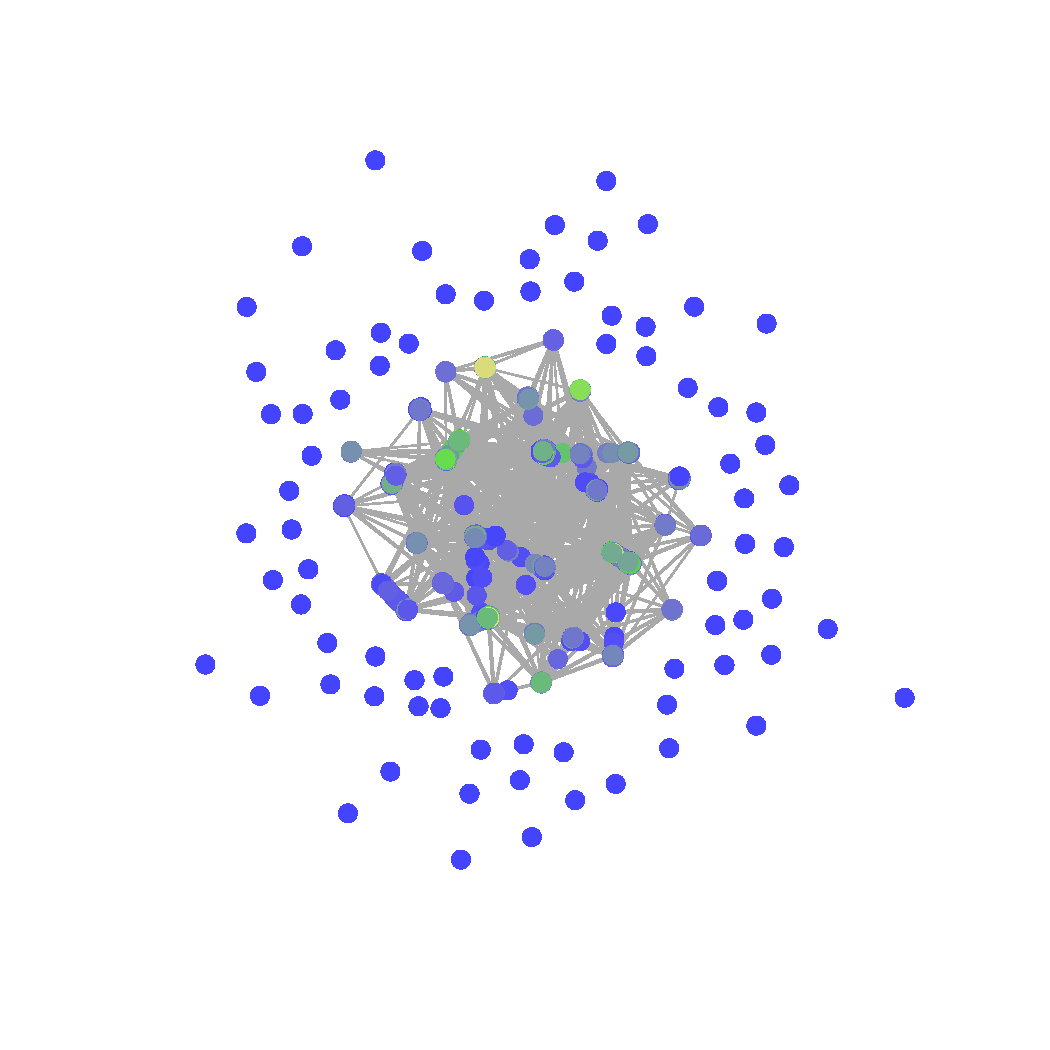
\includegraphics[width=.98\linewidth]{figure/all_actors-1} 

}

\caption[Visualization of Actors' Network]{Visualization of Actors' Network}\label{fig:all_actors}
\end{figure}


\end{knitrout}



In this section we plot the actors' network as a whole (see \Vref{fig:all_actors}).  For this plot, the node-size remained constant with the vertex color varying based on an actor's degree of connectedness (more blue for less connected and more red for well connected).  The data-set has 7015 actors in it.  The degree of connectedness in the set of actors is shown in \Vref{fig:actor_hist}.  This histogram shows that most actors have worked with between 40 and 60 other actors, although the heavy tail in this distribution indicates that many have worked with far more.  For instance ``Dobtcheff, Vernon'' has worked with 378 others.

\begin{knitrout}
\definecolor{shadecolor}{rgb}{0.969, 0.969, 0.969}\color{fgcolor}\begin{figure}

{\centering 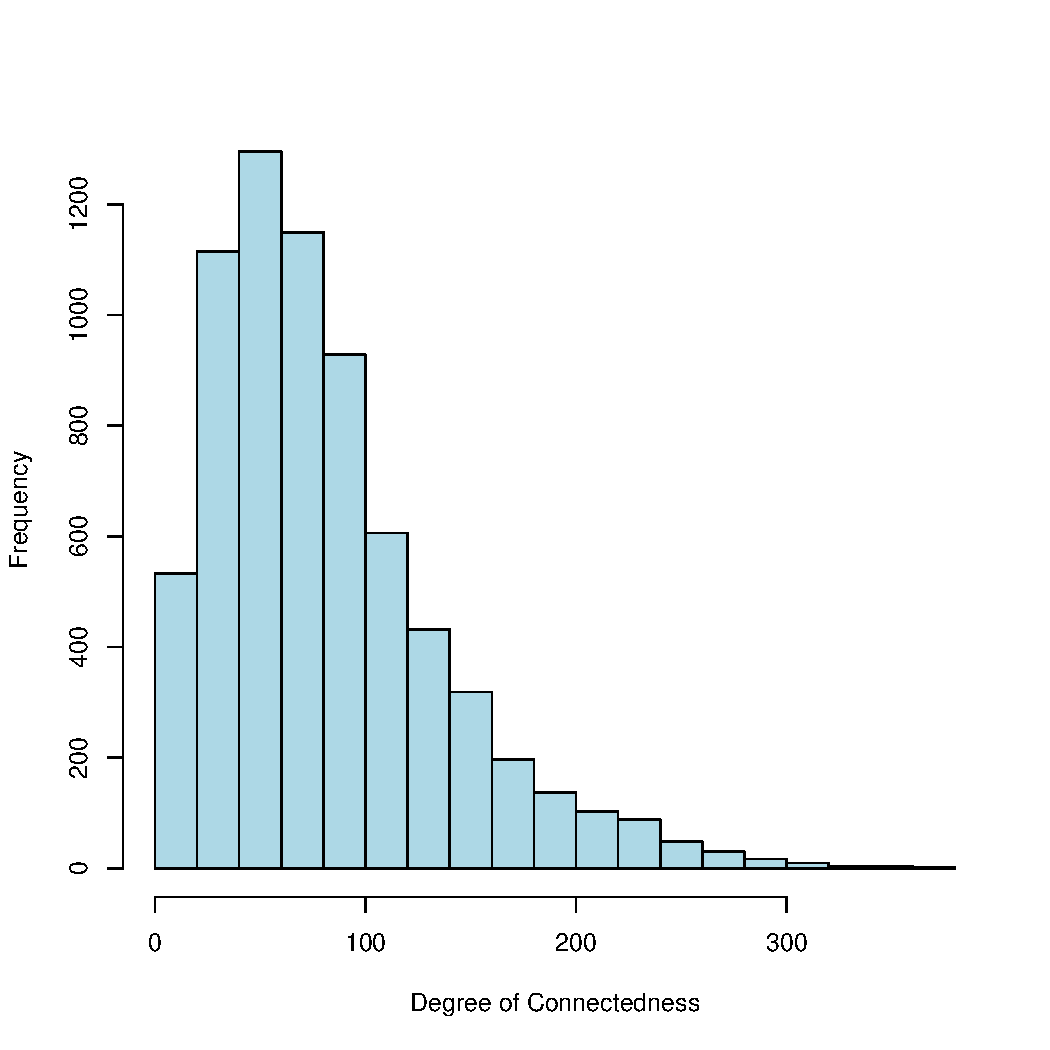
\includegraphics[width=.49\linewidth]{figure/actor_hist-1} 

}

\caption[Histogram of Actors' Connectedness]{Histogram of Actors' Connectedness}\label{fig:actor_hist}
\end{figure}


\end{knitrout}

\section{Kevin Bacon}


\begin{knitrout}
\definecolor{shadecolor}{rgb}{0.969, 0.969, 0.969}\color{fgcolor}\begin{figure}

{\centering \subfloat[1st Degree\label{fig:bacon1}]{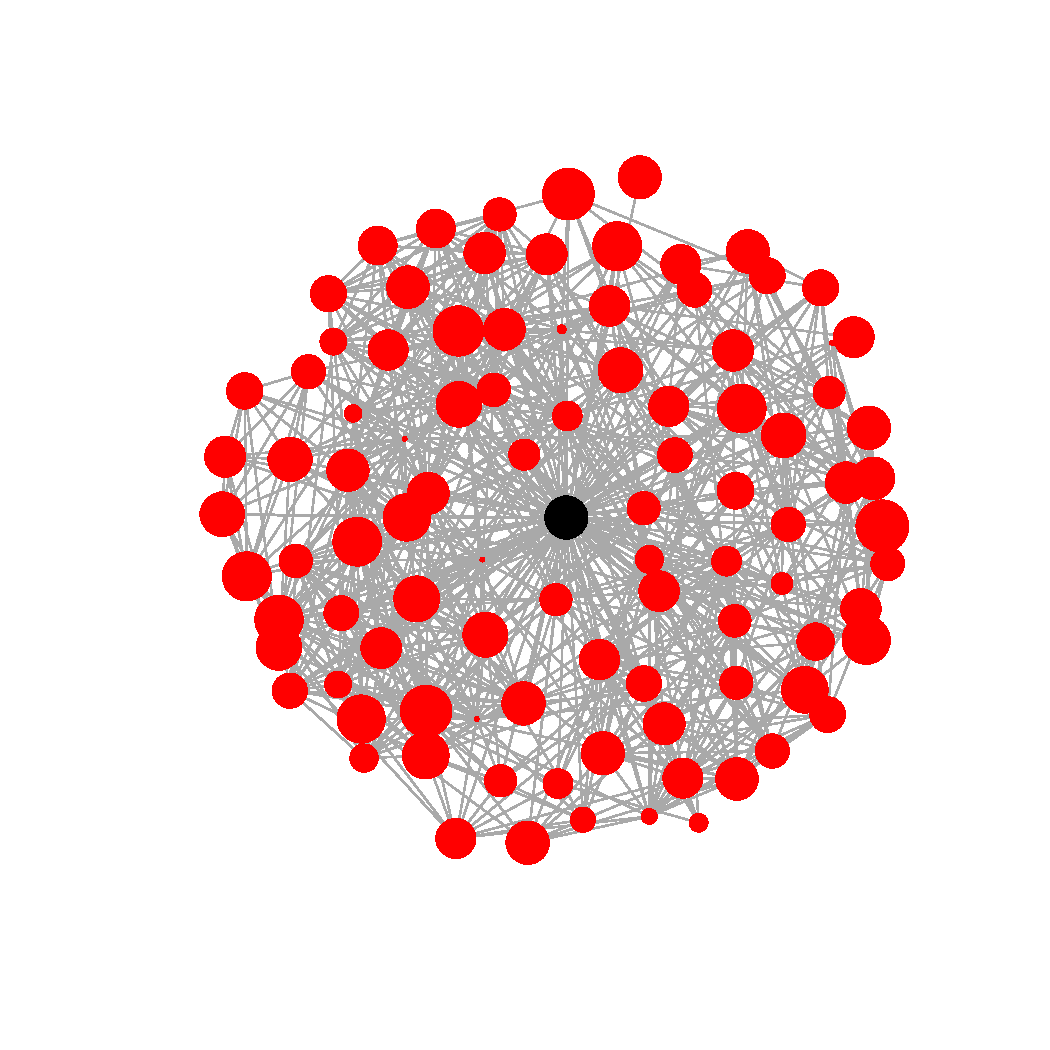
\includegraphics[width=.32\linewidth]{figure/bacon-1} }
\subfloat[2nd Degree\label{fig:bacon2}]{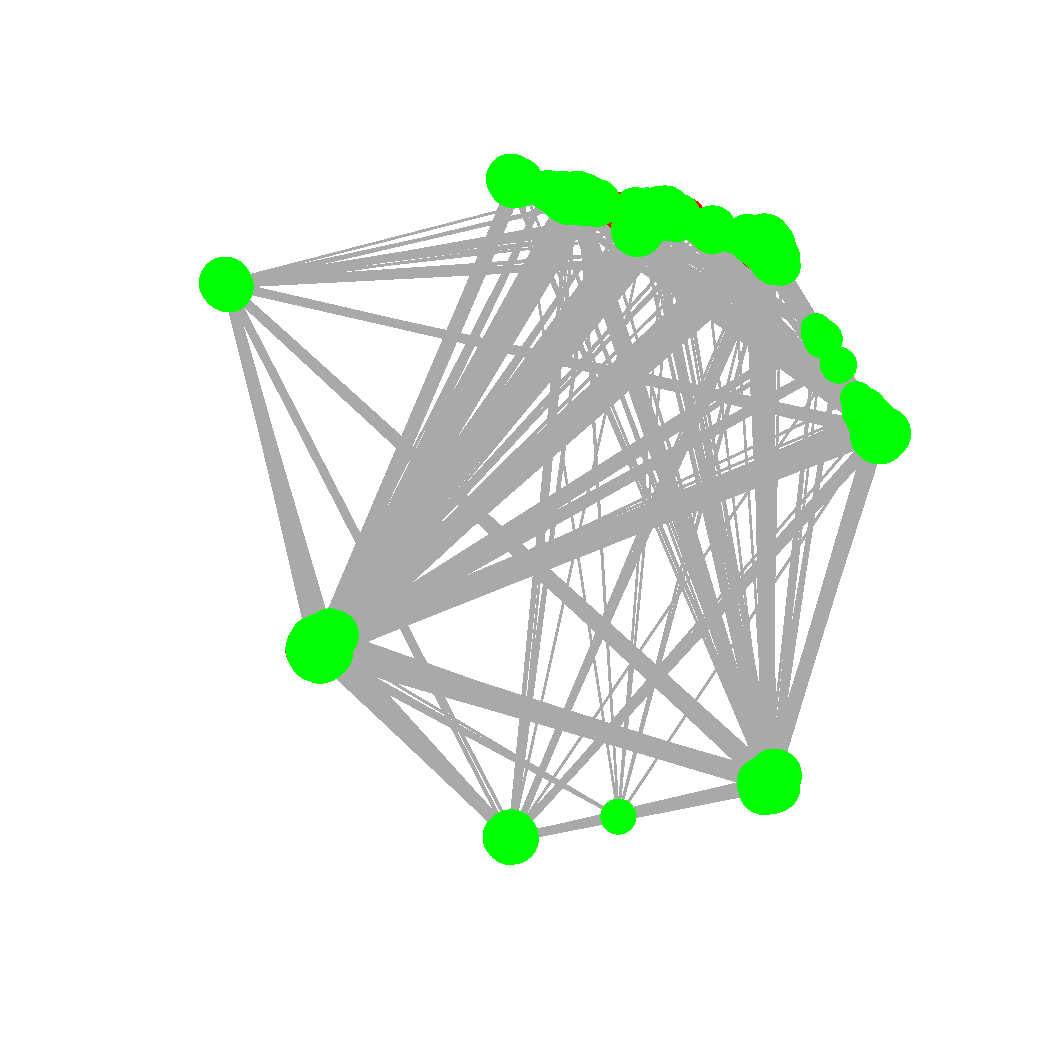
\includegraphics[width=.32\linewidth]{figure/bacon-2} }
\subfloat[3rd Degree\label{fig:bacon3}]{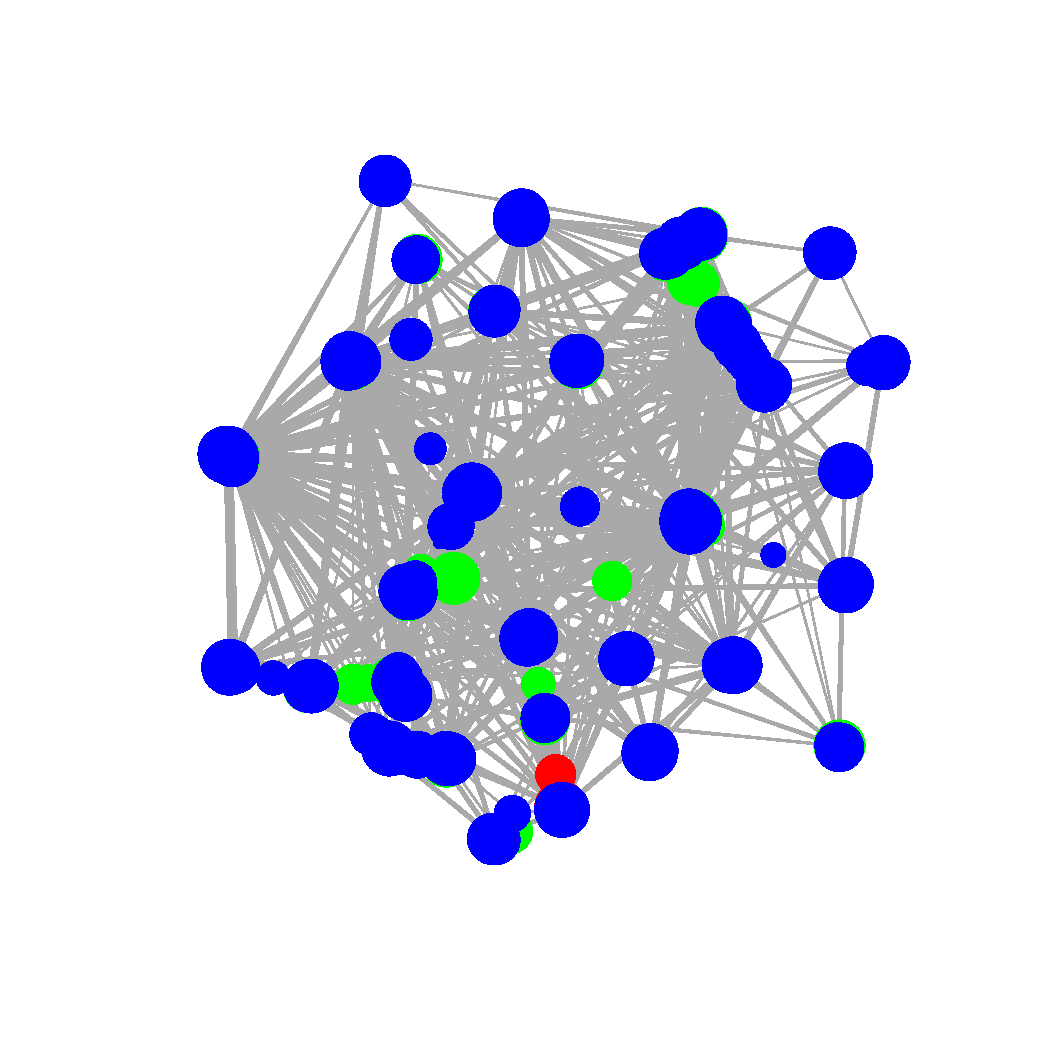
\includegraphics[width=.32\linewidth]{figure/bacon-3} }

}

\caption[Kevin Bacon's Network]{Kevin Bacon's Network}\label{fig:bacon}
\end{figure}


\end{knitrout}

Kevin Bacon's network can be visualized in \Vref{fig:bacon}.  In each of these plots, the node-size of each actor is sized according to their degree within the overall actors' network.  That is, larger degree actors have bigger nodes.  The coloring scheme used was to label 3rd-degree connections blue, 2nd-degree green, 1st-degree red, with Kevin Bacon's node colored black (see \Vref{r:bacon} for code used to generate these plots).



In \Cref{fig:bacon1} we see his 1st-degree connections and note that while Kevin Bacon is relatively well connected with 96 connections, 22.68\% of his connections have a higher degree than he does. In \Cref{fig:bacon2} we visualize 2nd-degree connections and note that of the 2128 connections, 27.99\% have a higher degree.  Also because of the way R rendered the visualization, we cannot really see any 1st degree conenctions.  In \Cref{fig:bacon3} we visualize 3rd-degree connections and see a much better visual dispersion of the three types of connections.  Of the 5980 connections, 31.23\% have more connections than Kevin Bacon.  

\section{Most Common and Connected Actors}




We can determine the most common actors by summing up the columns of the actors' matrix and sorting the result. The actor appearing in the most films is \textbf{Zivojinovic, Velimir 'Bata'}, who appeared in 57 films. The most connected actor is \textbf{Dobtcheff, Vernon}, who has been in at least one film with 378 other actors.



Here, we randomly select two actors \textbf{Auger, Claudine} and \textbf{Dray, Albert}. The shortest path between them contains 2 vertices: Auger, Claudine was in Secrets de la princesse de Cadignan, Les with  Arditi, Pierre ;, Arditi, Pierre was in Adieu blaireau with  Dray, Albert ;

\section{Appendix}
\begin{knitrout}
\definecolor{shadecolor}{rgb}{0.969, 0.969, 0.969}\color{fgcolor}\begin{kframe}
\begin{rlabel}\label{r:bacon}\hfill{}\begin{alltt}
\hlcom{# Generate actor vertex-sizes based on the degree of connectedness on the }
\hlcom{# overall actor network.  These constants were found by manually tuning the}
\hlcom{# size histogram.}
\hlstd{actorSizes} \hlkwb{<-} \hlnum{3}\hlopt{*}\hlkwd{log}\hlstd{(}\hlnum{0.5}\hlopt{*}\hlkwd{degree}\hlstd{(actnet)}\hlopt{+}\hlnum{1}\hlstd{)}\hlopt{+}\hlnum{1}

\hlcom{# Color the nodes for the 1st-degree plot}
\hlkwd{V}\hlstd{(actor1st)}\hlopt{$}\hlstd{color} \hlkwb{<-} \hlstr{"red"}
\hlkwd{V}\hlstd{(actor1st)[actor]}\hlopt{$}\hlstd{color} \hlkwb{<-} \hlstr{"black"}
\hlkwd{V}\hlstd{(actor1st)}\hlopt{$}\hlstd{frame.color} \hlkwb{<-} \hlkwd{V}\hlstd{(actor1st)}\hlopt{$}\hlstd{color}
\hlkwd{V}\hlstd{(actor1st)}\hlopt{$}\hlstd{size} \hlkwb{<-} \hlstd{actorSizes[}\hlkwd{V}\hlstd{(actor1st)]}
\hlkwd{plot}\hlstd{(actor1st,} \hlkwc{vertex.label}\hlstd{=}\hlnum{NA}\hlstd{,} \hlkwc{edge.curved}\hlstd{=F,} \hlkwc{margin}\hlstd{=}\hlnum{0}\hlstd{)}

\hlcom{# Color the nodes for the 2nd-degree plot}
\hlkwd{V}\hlstd{(actor2nd)}\hlopt{$}\hlstd{color} \hlkwb{<-} \hlstr{"green"}
\hlkwd{V}\hlstd{(actor2nd)[}\hlkwd{V}\hlstd{(actor1st)]}\hlopt{$}\hlstd{color} \hlkwb{<-} \hlstr{"red"}
\hlkwd{V}\hlstd{(actor2nd)[actor]}\hlopt{$}\hlstd{color} \hlkwb{<-} \hlstr{"black"}
\hlkwd{V}\hlstd{(actor2nd)}\hlopt{$}\hlstd{frame.color} \hlkwb{<-} \hlkwd{V}\hlstd{(actor2nd)}\hlopt{$}\hlstd{color}
\hlkwd{V}\hlstd{(actor2nd)}\hlopt{$}\hlstd{size} \hlkwb{<-} \hlstd{actorSizes[}\hlkwd{V}\hlstd{(actor2nd)]}
\hlkwd{plot}\hlstd{(actor2nd,} \hlkwc{vertex.label}\hlstd{=}\hlnum{NA}\hlstd{,} \hlkwc{edge.curved}\hlstd{=F,} \hlkwc{margin}\hlstd{=}\hlnum{0}\hlstd{)}

\hlcom{# Color the nodes for the 3rd-degree plot}
\hlkwd{V}\hlstd{(actor3rd)}\hlopt{$}\hlstd{color} \hlkwb{<-} \hlstr{"blue"}
\hlkwd{V}\hlstd{(actor3rd)[}\hlkwd{V}\hlstd{(actor2nd)]}\hlopt{$}\hlstd{color} \hlkwb{<-} \hlstr{"green"}
\hlkwd{V}\hlstd{(actor3rd)[}\hlkwd{V}\hlstd{(actor1st)]}\hlopt{$}\hlstd{color} \hlkwb{<-} \hlstr{"red"}
\hlkwd{V}\hlstd{(actor3rd)[actor]}\hlopt{$}\hlstd{color} \hlkwb{<-} \hlstr{"black"}
\hlkwd{V}\hlstd{(actor3rd)}\hlopt{$}\hlstd{frame.color} \hlkwb{<-} \hlkwd{V}\hlstd{(actor3rd)}\hlopt{$}\hlstd{color}
\hlkwd{V}\hlstd{(actor3rd)}\hlopt{$}\hlstd{size} \hlkwb{<-} \hlstd{actorSizes[}\hlkwd{V}\hlstd{(actor3rd)]}
\hlkwd{plot}\hlstd{(actor3rd,} \hlkwc{vertex.label}\hlstd{=}\hlnum{NA}\hlstd{,} \hlkwc{edge.curved}\hlstd{=F,} \hlkwc{margin}\hlstd{=}\hlnum{0}\hlstd{)}
\end{alltt}
\end{rlabel}\end{kframe}
\end{knitrout}

\end{document}
